\documentclass{article}
\usepackage{graphicx}
\usepackage[margin=1.5cm]{geometry}
\usepackage{amsmath}
\usepackage{fancyvrb}
\usepackage{url}

\begin{document}

\title{Synopsis - Week 0: Introduction and Laboratory Tour}
\author{Prof. Jordan C. Hanson}

\maketitle

\section{Review of DC Circuits}

\begin{enumerate}
\item Suppose a DC circuit is constructed by connecting a switch and a device with resistance 1 k$\Omega$ in series with a 5 V battery.  How much current will flow if the switch is closed?  Draw a diagram of the circuit.  \\ \vspace{1cm}
\item Suppose two 330 $\Omega$ resistors are connected in parallel.  (a) What is the total effective resistance?  (b) Suppose two 330 $\Omega$ resistors are connected in series.  (c) If connected to a 5V source, forming a circuit, how much current will flow?   (d) What will be the power dissipated in the circuit?\\ \vspace{1cm}
\end{enumerate}

\section{Introduction to PYNQ-Z1 System-on-a-Chip (SoC)}

\begin{enumerate}
\item Let's review \url{https://youtu.be/SuXkbcK3w9E} for an introduction to our SoC.
\begin{figure}
\centering
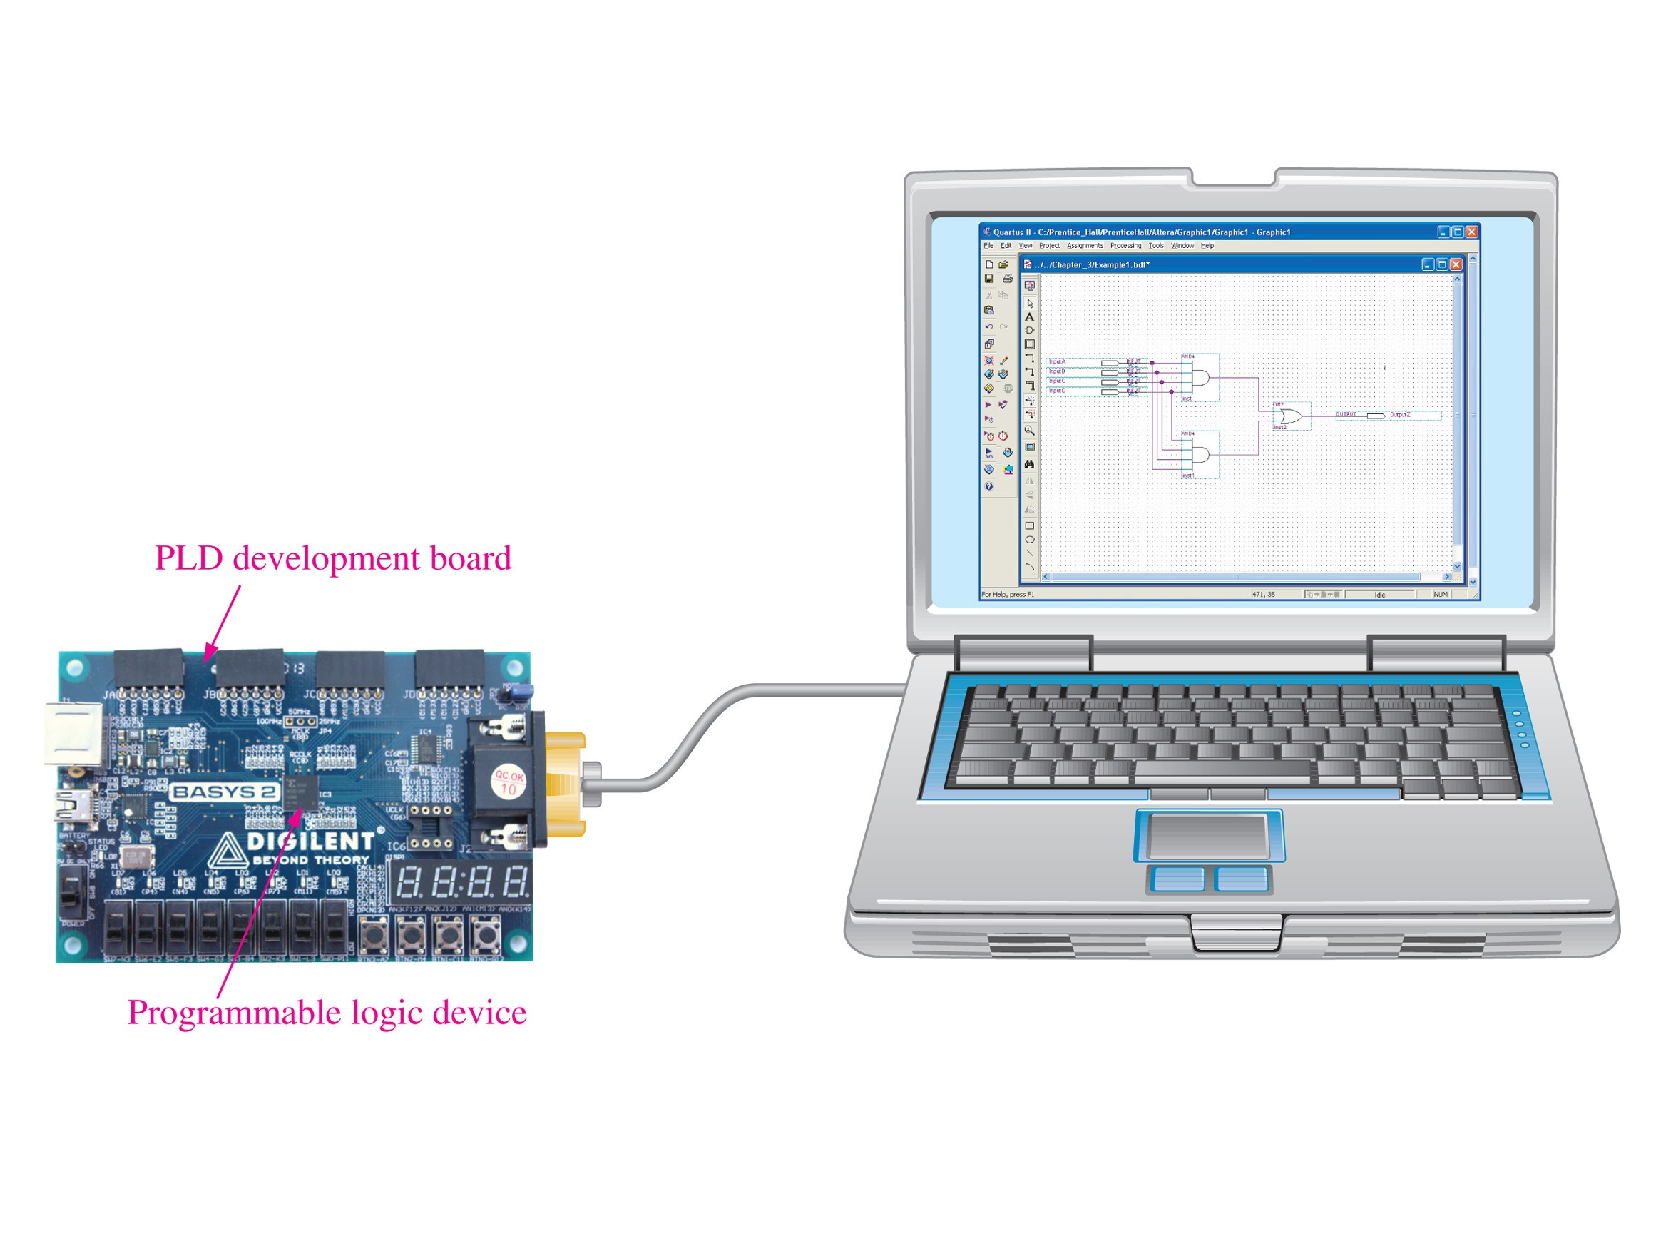
\includegraphics[width=0.35\textwidth]{PYNQandLaptop.pdf}
\caption{\label{fig:pynq} The setup of using a laptop to program a PLD development board.}
\end{figure}
\item (Select lab partners).  Take a seat at one of the laptops in the lab.  Power it up, and at the login prompt, type \verb+cosc330+ as the password.  Use the Menu at lower left to find a program called ``terminal.''  Type the commands \verb+ls+, \verb+pwd+, and \verb+find+.  What is the purpose of each?  Type \verb+man find+ to open the manual for the \verb+find+ command.  
\begin{itemize}
\item ls:
\item pwd:
\item find:
\end{itemize}
\item Connect the PYNQ-Z1 board to the laptop via the USB to Ethernet converter.  Next, connect the micro-USB cable between the PYNQ-Z1 and the laptop.  Open a browser and navigate to http://192.168.2.99.
\item You should be prompted to enter a password.  Type \verb+xilinx+.  You are now inside the chip at the center of the board, running a version of linux on the dual-core ARM.  Navigate to the Getting Started folder by clicking, and run the tutorial entitled \verb+1_jupyter_notebook.ipynb+.  Python notebooks can run code and contain writing in markup.
\item Click the ``Running'' tab when you are done with the notebook, and close the jupyter notebook.  Click ``New'' in the upper right hand corner to open a terminal.  In the terminal, type \verb+shutdown now+.  Close the browser tabs and power down the PYNQ-Z1 board.
\end{enumerate}

\section{Introduction to Test and Measurement Instruments}

\begin{enumerate}
\item Our first instrument to learn is the oscilloscope and function generator.  These two pieces of test equipment are incorporated into one device in this application.  Connect the BNC coaxial cable (the black cable) between the \verb+Gen+ output and channel 1\footnote{This feature is not enabled on every scope.  Please double up in groups to observe if the scope gives you an error message.}.  Press the Wave Gen button under Trigger.  Determine how to create a sine wave signal by tuning the parameters at the bottom.
\begin{figure}
\centering
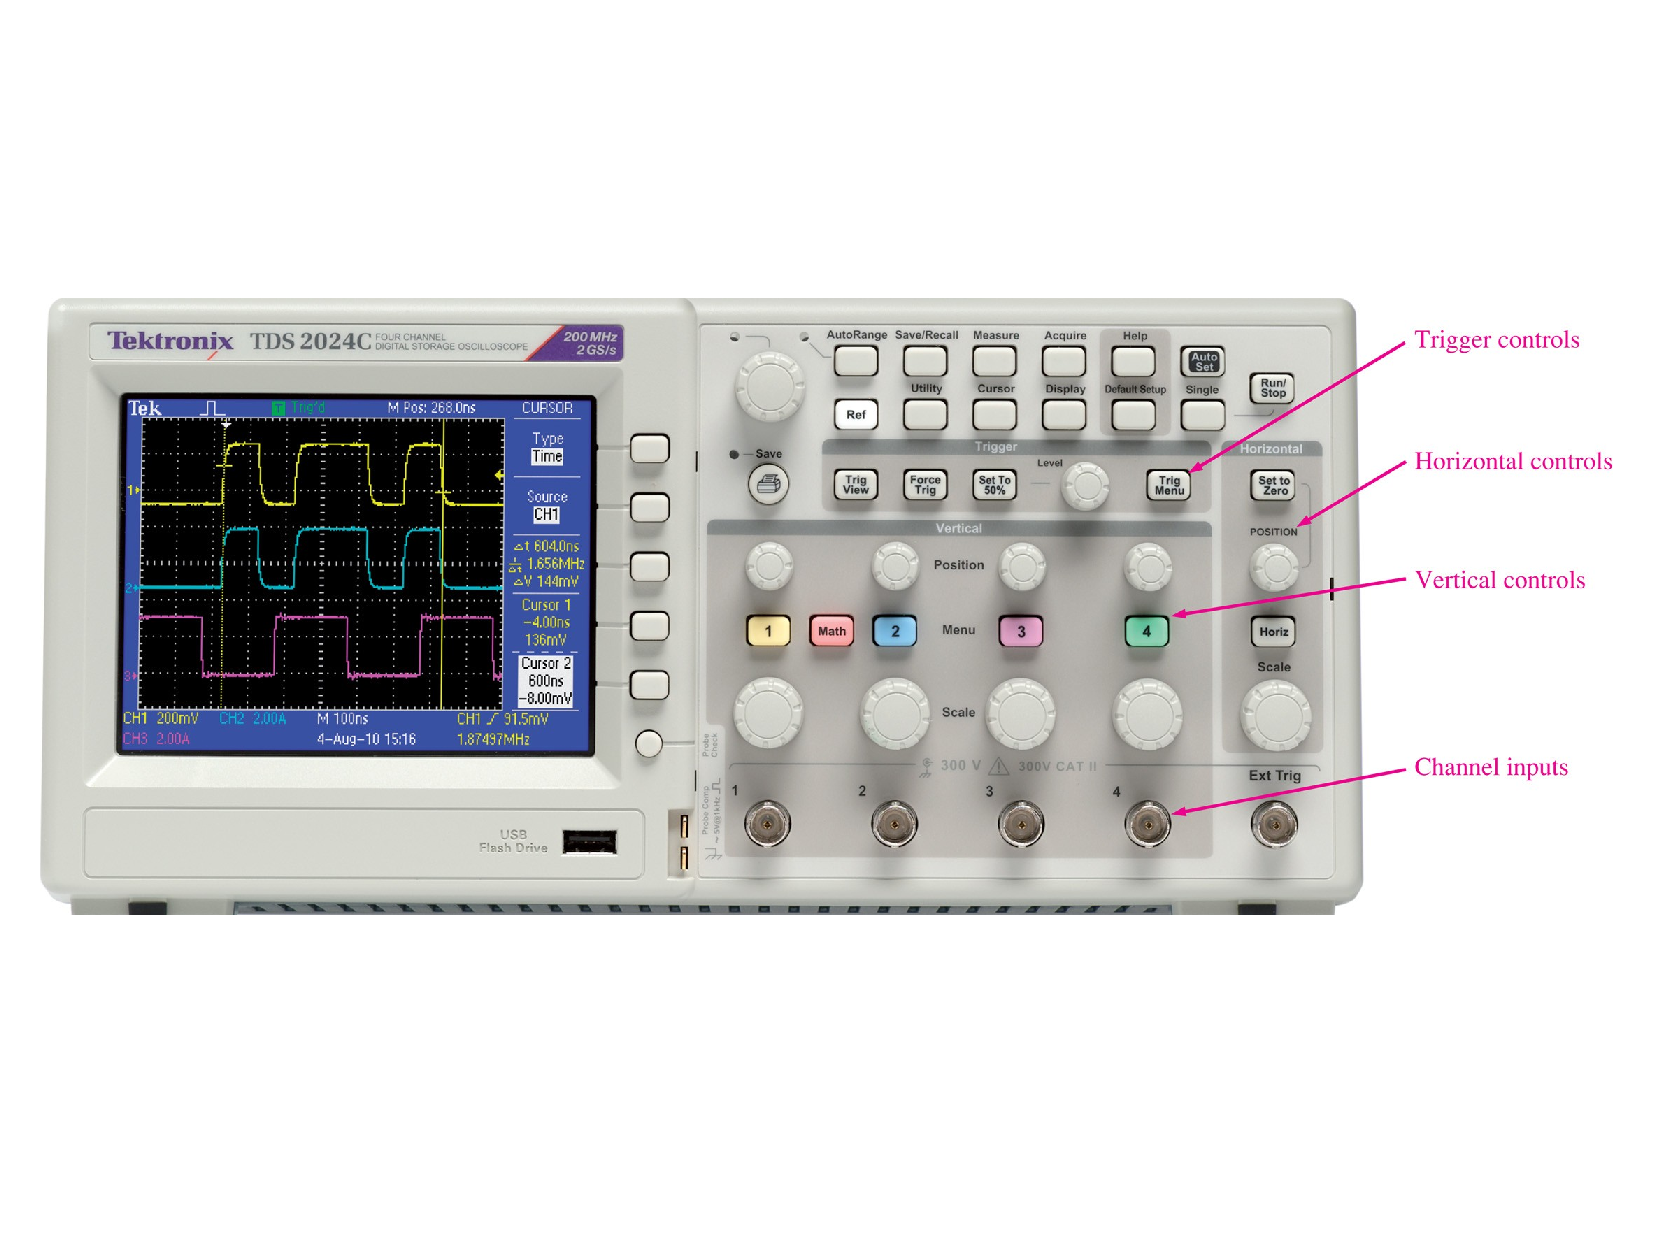
\includegraphics[width=0.55\textwidth,trim=0cm 5cm 0cm 5cm,clip=true]{Scope.pdf}
\caption{\label{fig:scope} The basic controls of an oscilloscope  This model is not exactly the same one as those in the lab, but the features are identical.}
\end{figure}
\item Remember the amplitude in volts of the sine wave, and adjust the trigger voltage with the grey knob under trigger until the waveform is displayed.
\item Select ``Pulse'' from the signal types, and set the frequency to 1 kHz.  Set the high level to some voltage above 100 mV, and the low voltage to 0.0 V (these controls are along the bottom).  Adjust the pulse width to 100 $\mu$s, giving the pulse a \textit{duty cycle} of 10 \%.  Make sure you are still triggering on it.
\item Zoom in on one of the pulses, presumably the one on which the scope is triggering.  Sketch it below, noting how the features differ from a perfect square pulse.
\end{enumerate}

\end{document}
